
\documentclass{report}

\usepackage[utf8]{inputenc}
\usepackage[italian]{babel}
\usepackage{import}
\usepackage{todonotes}
\usepackage{color}
\usepackage{rotating}
\usepackage[hidelinks]{hyperref}
\usepackage{url}
\usepackage{pdfpages}
\usepackage{siunitx}
\usepackage{pdflscape}
\usepackage{subfig}
\usepackage[euler]{textgreek}
\usepackage{mhchem}

\usepackage{multirow}

\usepackage{enumerate} 
\usepackage{amsmath}
\usepackage{amsfonts}

\usepackage[signatures,swapnames,sans]{frontespizio}

\usepackage{geometry}
\geometry{portrait, margin=3cm}
\usepackage{siunitx}
\usepackage{booktabs}

\renewcommand*\figurename{Figura}

\newcommand{\sub}[1]{\textsubscript{#1}}
\newcommand{\super}[1]{\textsuperscript{#1}}
\newcommand{\parallelsum}{\mathbin{\!/\mkern-5mu/\!}}

\newcommand{\Fig}[0]{Fig.}

\usepackage{titlesec}

\titleformat{\chapter}{\normalfont\huge}{}{20pt}{\huge\bfseries}

\linespread{1.3}


%% COMANDI UTILI
%\begin{table}[h]
%	\centering
%	\begin{tabular}{|c|c|c|}
%	\cline{2-3} 
%	\multicolumn{1}{c|}{} & \textbf{Valore nominale} & \textbf{Valore misurato}\\ 
%		%\hline
%		%{} & \textbf{Valore nominale} & \textbf{Valore misurato} \\ 
%		\hline
%		$\mathbf{R_1}$ & \SI{18}{k\ohm} & \SI{17.977}{k\ohm} \\ 
%		\hline
%		$\mathbf{R_2}$& \SI{1.8}{k\ohm} & \SI{1.815}{k\ohm} \\ 
%		\hline
%	\end{tabular}
%\caption{Misure delle resistenze utilizzate per il circuito.}
%\label{table:mis_res}
%\end{table}
%\begin{figure}[h!]
%\centering
%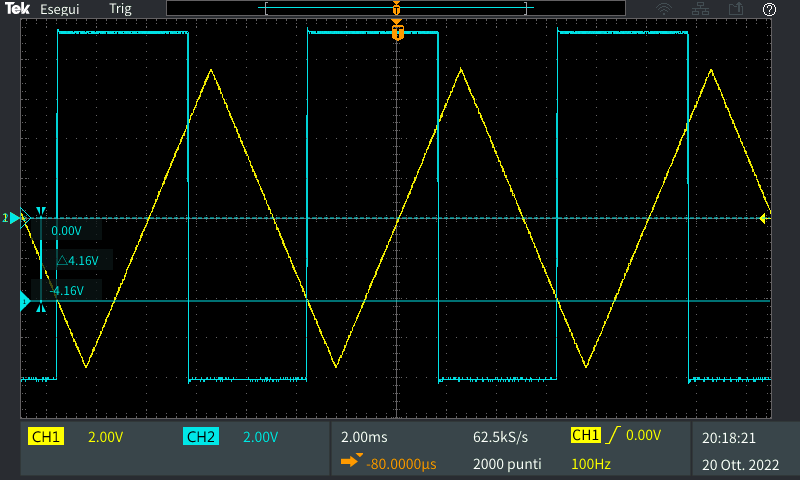
\includegraphics[height=6.5cm]{immagini/TEK00018}\\(a)\\[1ex]
%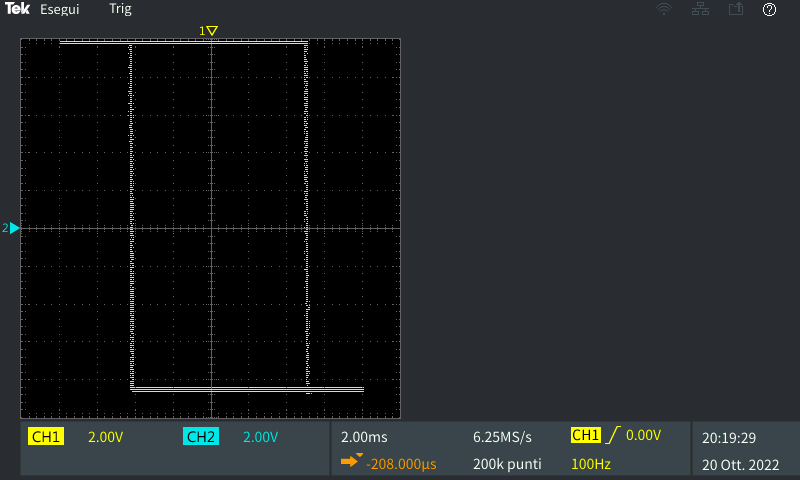
\includegraphics[height=6.5cm]{immagini/TEK00019}\\(b)
%\caption{Risposta del circuito con accoppiamento DC (a) e accoppiamento AC (b).}
%	\label{figura:accopp}
%\end{figure}

\begin{document}
\addtocounter{chapter}{+2}
	\begin{frontespizio}
		\Margini{3cm}{3cm}{3cm}{3cm}
		\Universita{Bergamo}
		\Logo[43.332mm]{unibg-mark}
		\Divisione{Scuola di Ingegneria}
		\Corso[Laurea Magistrale]{Ingegneria Informatica}
		\Titolo{Laboratorio di Elettronica}
		\Sottotitolo{Relazione esperienza di laboratorio 3}
		\Punteggiatura{}
		\NRelatore{Prof.}{Prof.}
		\Relatore{Luigi Gaioni}
		\Candidato[1058231]{Giulia Allievi}
		\Candidato[1059640]{Martina Fanton}
		\Annoaccademico{2022--2023}
		\begin{Preambolo*}
			\usepackage[italian]{babel}
			\usepackage[T1]{fontenc}
			\usepackage[utf8]{inputenc}
			\usepackage{microtype}
			\usepackage{lmodern}
			\graphicspath{{img/}}
			
			\renewcommand{\frontinstitutionfont}{\fontsize{14}{17}\bfseries\scshape}
			\renewcommand{\fronttitlefont}{\fontsize{17}{21}\bfseries\scshape}
			\renewcommand{\frontfootfont}{\fontsize{12}{14}\bfseries\scshape}
		\end{Preambolo*}
	\end{frontespizio}

%----------------------------------------------------------------------------------------
%	PAGINA BIANCA
%----------------------------------------------------------------------------------------
\newpage
\null
\thispagestyle{empty}
\newpage

%----------------------------------------------------------------------------------------
%	INTRO
%----------------------------------------------------------------------------------------
\chapter{Relazione attività di laboratorio 3}
\section*{Introduzione}
\newpage
\section{Circuito 1: raddrizzatore a doppia semionda di precisione}
\subsection{Schema del circuito e Funzione di Trasferimento}
\begin{figure}[h]
	\centering
	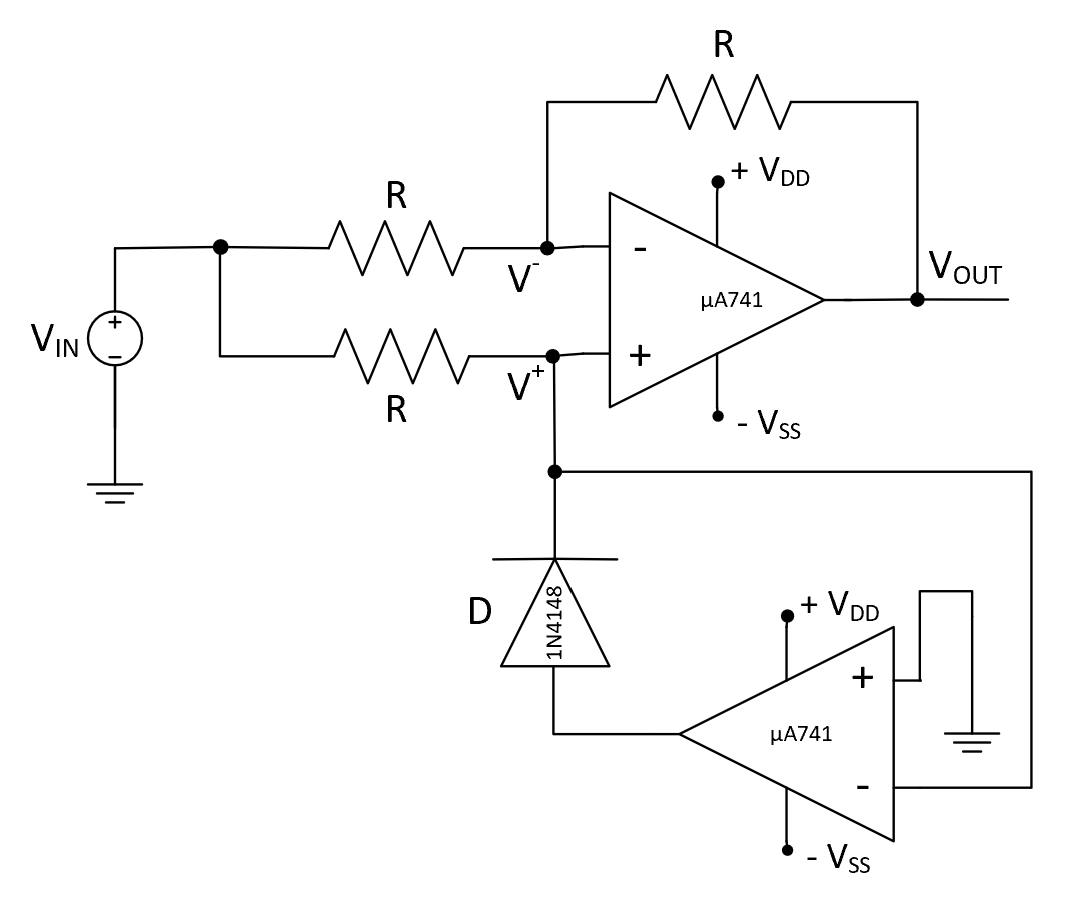
\includegraphics[height=6.2cm]{immagini/schema1}
	\caption{Schema del raddrizzatore a doppia semionda di precisione.}
	\label{figura:schema1}
\end{figure}
\noindent La funzione di trasferimento di questo raddrizzatore è:
\begin{equation}
   \begin{cases}
   V_{in}< \SI{0}{\volt}\;\;\indent\indent\rightarrow \mathrm{D\;ON}\;\;\;\; \Rightarrow V_{out} = -V_{in}\\
   V_{in}\ge \SI{0}{\volt}\;\;\indent\indent\rightarrow \mathrm{D\; OFF}\;\; \Rightarrow V_{out} = V_{in}
   \end{cases}
\end{equation}
\subsection{Analisi e dati sperimentali}
\begin{figure}[h]
	\centering
	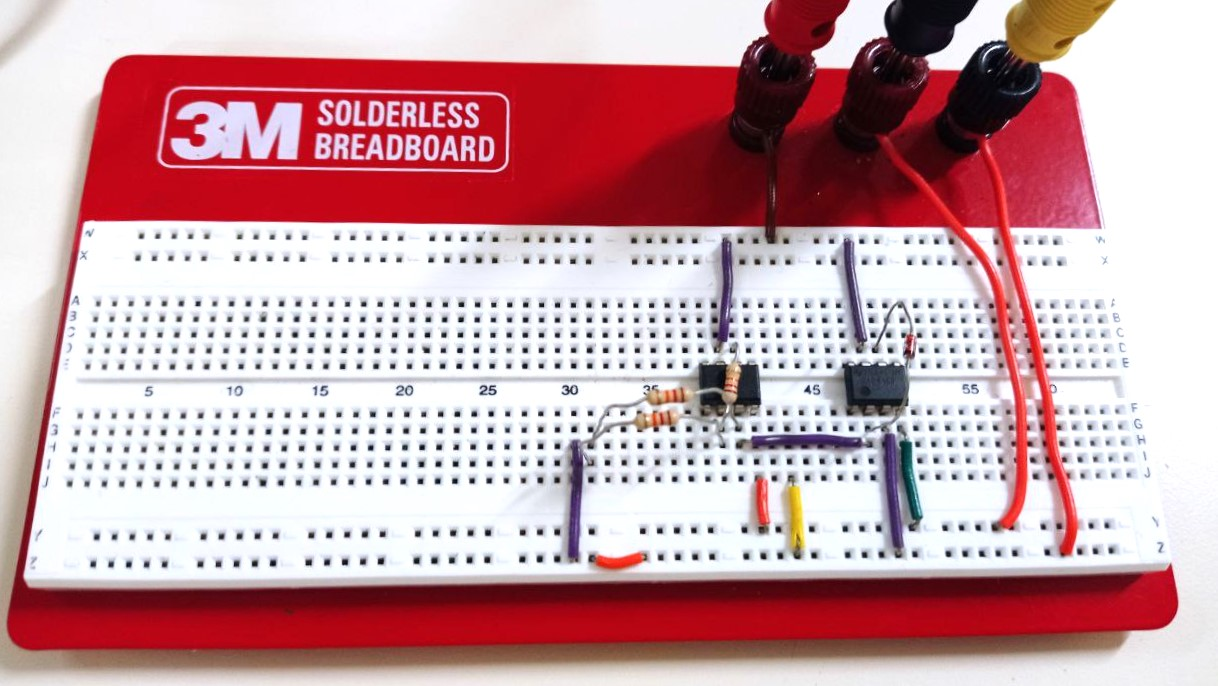
\includegraphics[height=6.2cm]{immagini/circuito1}
	\caption{Fotografia del raddrizzatore a doppia semionda di precisione realizzato in laboratorio.}
	\label{figura:circuito1}
\end{figure}
%\begin{table}[h!]
%	\centering
%	\begin{tabular}{|c|c|c|}
%		\cline{2-3} 
%		\multicolumn{1}{c|}{} & \textbf{Valore nominale} & \textbf{Valore misurato}\\ 
%		\hline
%		$\mathbf{R_1}$ & \SI{18}{k\ohm} & \SI{17.977}{k\ohm} \\ 
%		\hline
%		$\mathbf{R_2}$ & \SI{33}{k\ohm} & \SI{37.630}{k\ohm} \\ 
%		\hline
%		$\mathbf{R_3}$ & \SI{56}{k\ohm} & \SI{54.742}{k\ohm} \\ 
%		\hline
%		$\mathbf{R_4}$ & $\displaystyle\mathrm{\SI{82}{k\ohm}+\SI{18}{k\ohm}=\SI{100}{k\ohm}}$ & $\displaystyle\mathrm{\SI{80.717}{k\ohm+}\SI{17.977}{k\ohm}=\SI{98.694}{k\ohm}}$ \\ 
%		\hline
%	\end{tabular}
%	\caption{Misure delle resistenze utilizzate nel raddrizzatore a semionda passivo.}
%	\label{table:misure1}
%\end{table}

\section{Circuito 2: trigger di Schmitt}
\subsection{Schema del circuito e Funzione di Trasferimento}
\begin{figure}[h]
	\centering
	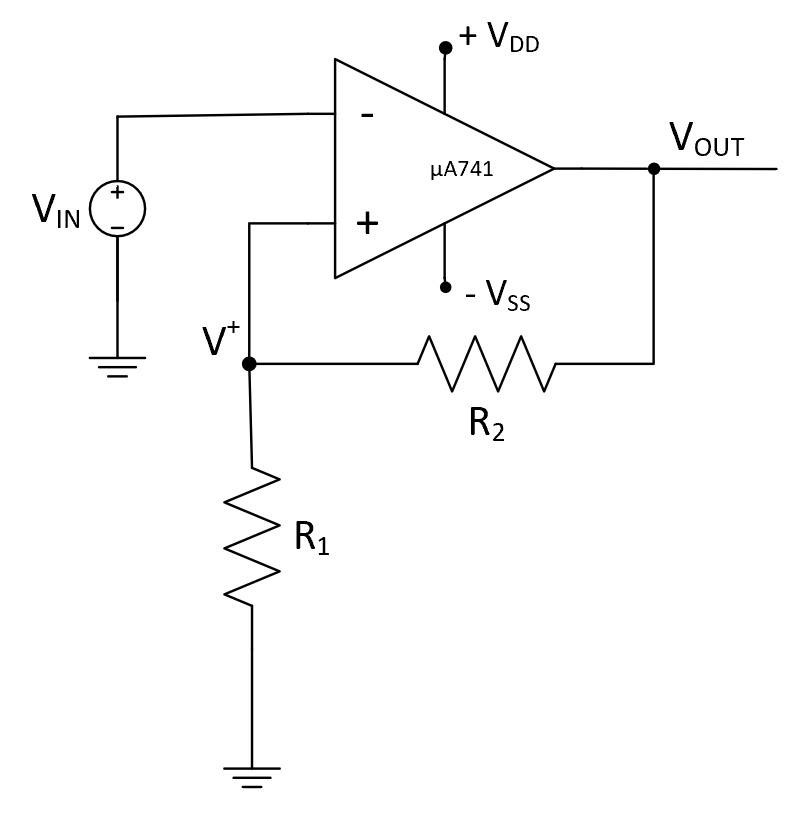
\includegraphics[height=6.2cm]{immagini/schema2}
	\caption{Schema del trigger di Schmitt.}
	\label{figura:schema2}
\end{figure}
\noindent La funzione di trasferimento di questo comparatore è:
\begin{equation}
   \begin{cases} % da controllare
   V_{out}= V_{DD}\;\indent\indent \mathrm{per\;}  V_L^+<V_{in}<V_H^+\mathrm{, \;\; con\;}\displaystyle{ V_H^+=\frac{R_1}{R_1+R_2}\cdot V_{DD}=\frac{V_{DD}}{2}}\mathrm{\;\;\;\; se \;} R_1=R_2\\[10pt]
   V_{out}= V_{SS}\;\;\indent\indent \mathrm{per\;} V_H^+<V_{in}<V_L^+\mathrm{, \;\; con\;}\displaystyle{ V_H^+=\frac{R_1}{R_1+R_2}\cdot |V_{SS}|=\frac{|V_{SS}|}{2}}\mathrm{\;\; se \;} R_1=R_2\\
   \end{cases}
\end{equation}
\subsection{Analisi e dati sperimentali}
\begin{figure}[h]
	\centering
	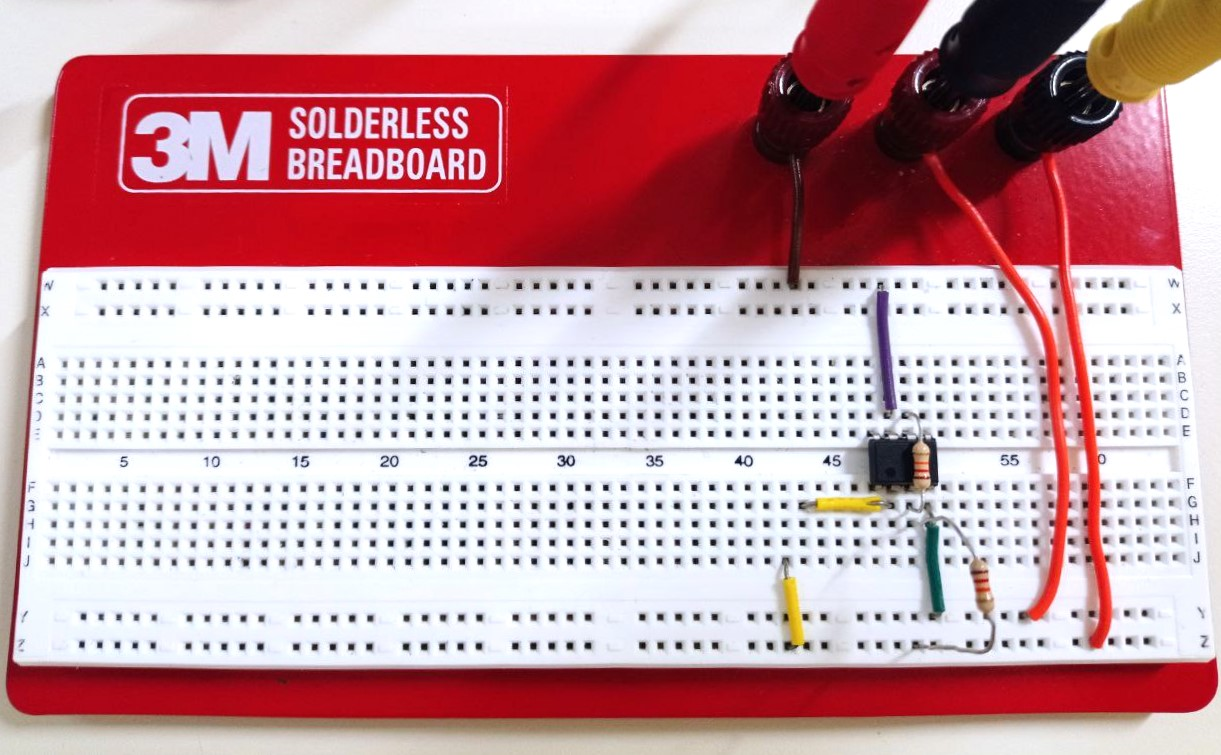
\includegraphics[height=6.2cm]{immagini/circuito2}
	\caption{Fotografia del trigger di Schmitt realizzato in laboratorio.}
	\label{figura:circuito2}
\end{figure}
%\begin{table}[h!]
%	\centering
%	\begin{tabular}{|c|c|c|}
	%		\cline{2-3} 
	%		\multicolumn{1}{c|}{} & \textbf{Valore nominale} & \textbf{Valore misurato}\\ 
	%		\hline
	%		$\mathbf{R_1}$ & \SI{18}{k\ohm} & \SI{17.977}{k\ohm} \\ 
	%		\hline
	%		$\mathbf{R_2}$ & \SI{33}{k\ohm} & \SI{37.630}{k\ohm} \\ 
	%		\hline
	%		$\mathbf{R_3}$ & \SI{56}{k\ohm} & \SI{54.742}{k\ohm} \\ 
	%		\hline
	%		$\mathbf{R_4}$ & $\displaystyle\mathrm{\SI{82}{k\ohm}+\SI{18}{k\ohm}=\SI{100}{k\ohm}}$ & $\displaystyle\mathrm{\SI{80.717}{k\ohm+}\SI{17.977}{k\ohm}=\SI{98.694}{k\ohm}}$ \\ 
	%		\hline
	%	\end{tabular}
%	\caption{Misure delle resistenze utilizzate nel raddrizzatore a semionda passivo.}
%	\label{table:misure1}
%\end{table}

\section{Circuito 3: oscillatore con duty cicle = 50\%}
\subsection{Schema del circuito e Funzione di Trasferimento}
\begin{figure}[h]
	\centering
	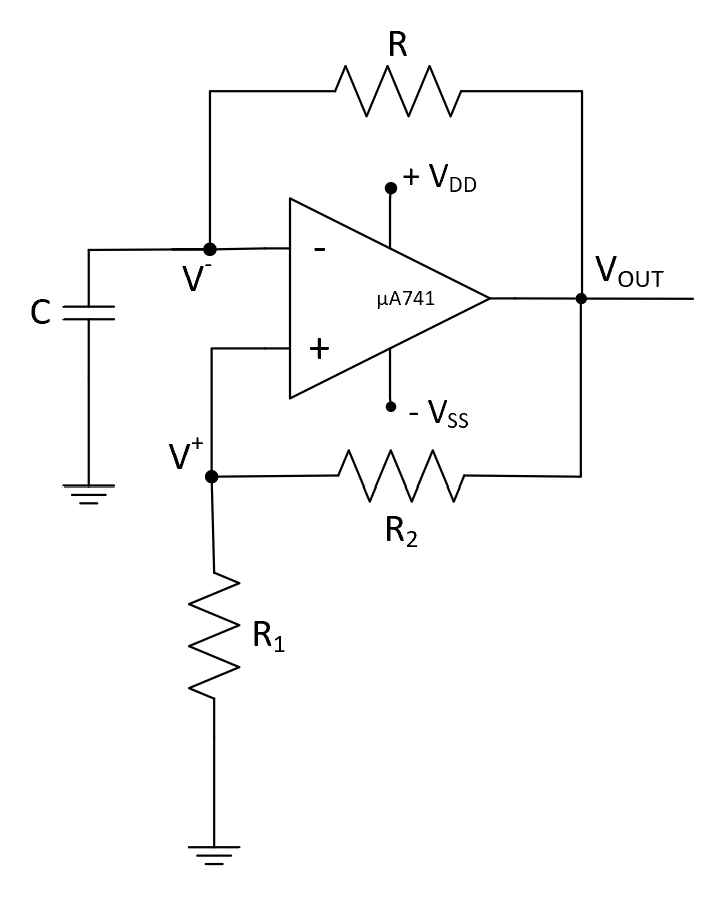
\includegraphics[height=6.2cm]{immagini/schema3}
	\caption{Schema dell'oscillatore con duty cicle = 50\%.}
	\label{figura:schema3}
\end{figure}
%\noindent La funzione di trasferimento di questo raddrizzatore è:
%\begin{equation}
%   \begin{cases}
	%   \end{cases}
%\end{equation}
\subsection{Analisi e dati sperimentali}
\begin{figure}[h]
	\centering
	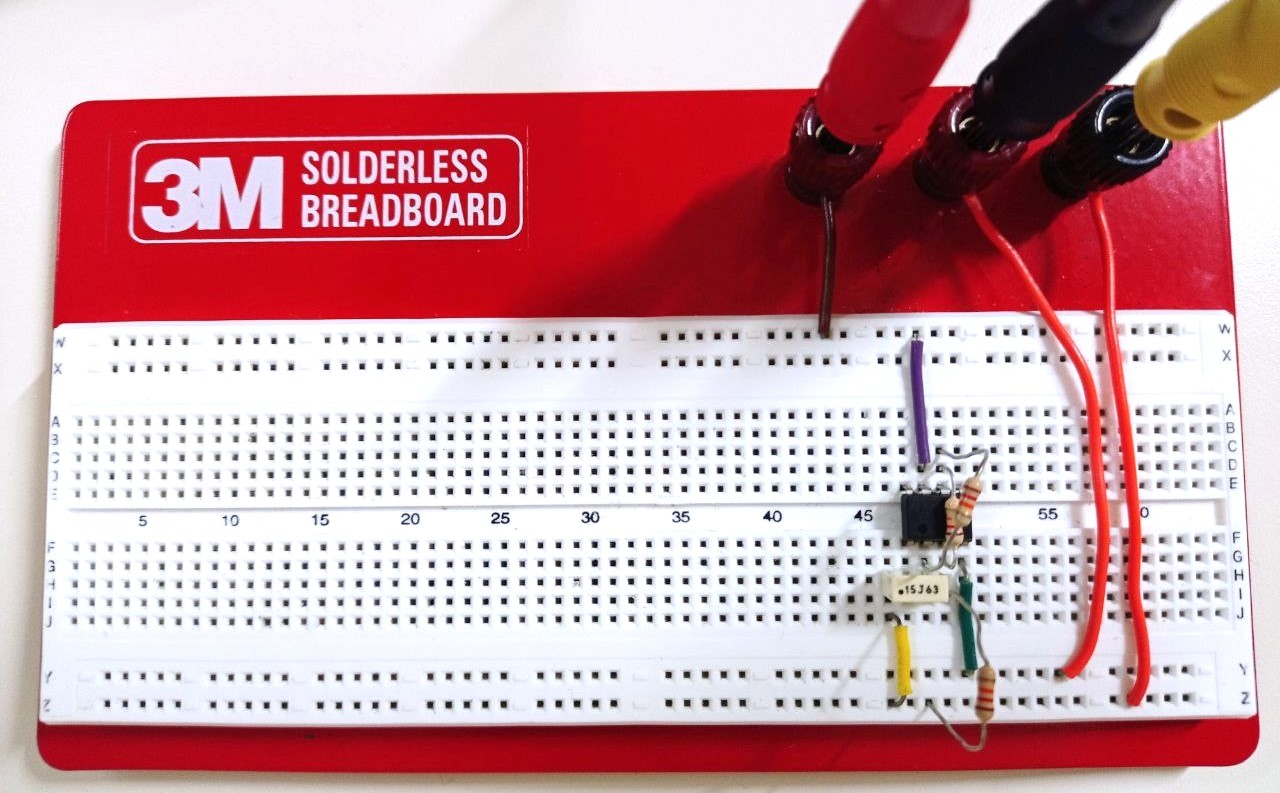
\includegraphics[height=6.2cm]{immagini/circuito3}
	\caption{Fotografia dell'oscillatore con duty cicle = 50\% realizzato in laboratorio.}
	\label{figura:circuito3}
\end{figure}
%\begin{table}[h!]
%	\centering
%	\begin{tabular}{|c|c|c|}
	%		\cline{2-3} 
	%		\multicolumn{1}{c|}{} & \textbf{Valore nominale} & \textbf{Valore misurato}\\ 
	%		\hline
	%		$\mathbf{R_1}$ & \SI{18}{k\ohm} & \SI{17.977}{k\ohm} \\ 
	%		\hline
	%		$\mathbf{R_2}$ & \SI{33}{k\ohm} & \SI{37.630}{k\ohm} \\ 
	%		\hline
	%		$\mathbf{R_3}$ & \SI{56}{k\ohm} & \SI{54.742}{k\ohm} \\ 
	%		\hline
	%		$\mathbf{R_4}$ & $\displaystyle\mathrm{\SI{82}{k\ohm}+\SI{18}{k\ohm}=\SI{100}{k\ohm}}$ & $\displaystyle\mathrm{\SI{80.717}{k\ohm+}\SI{17.977}{k\ohm}=\SI{98.694}{k\ohm}}$ \\ 
	%		\hline
	%	\end{tabular}
%	\caption{Misure delle resistenze utilizzate nel raddrizzatore a semionda passivo.}
%	\label{table:misure1}
%\end{table}

\section{Circuito 4: oscillatore con duty cicle $\neq$ 50\%}
\subsection{Schema del circuito e Funzione di Trasferimento}
\begin{figure}[h]
	\centering
	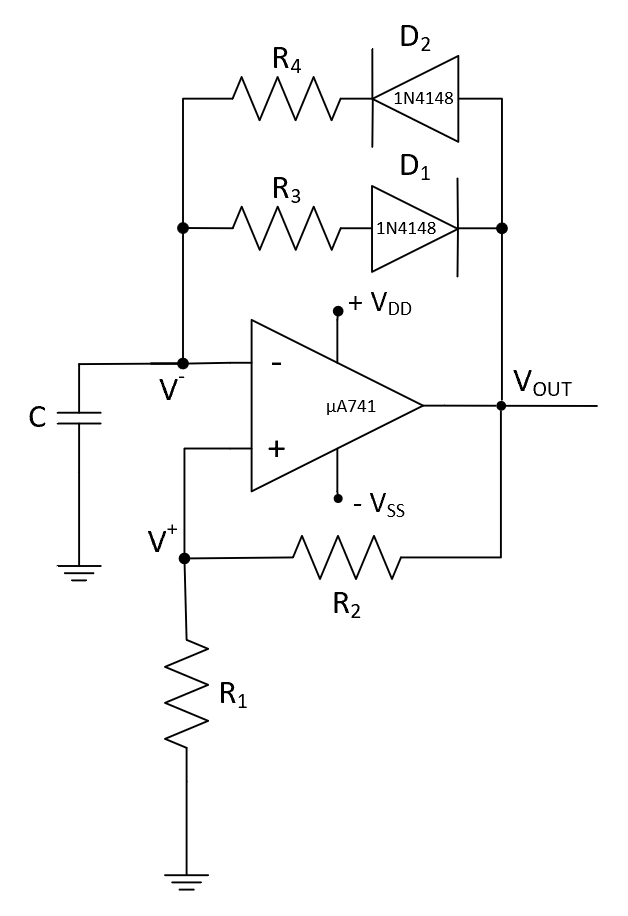
\includegraphics[height=6.2cm]{immagini/schema4}
	\caption{Schema dell'oscillatore con duty cicle $\neq$ 50\%.}
	\label{figura:schema4}
\end{figure}
%\noindent La funzione di trasferimento di questo raddrizzatore è:
%\begin{equation}
%   \begin{cases}
	%   \end{cases}
%\end{equation}
\subsection{Analisi e dati sperimentali}
\begin{figure}[h]
	\centering
	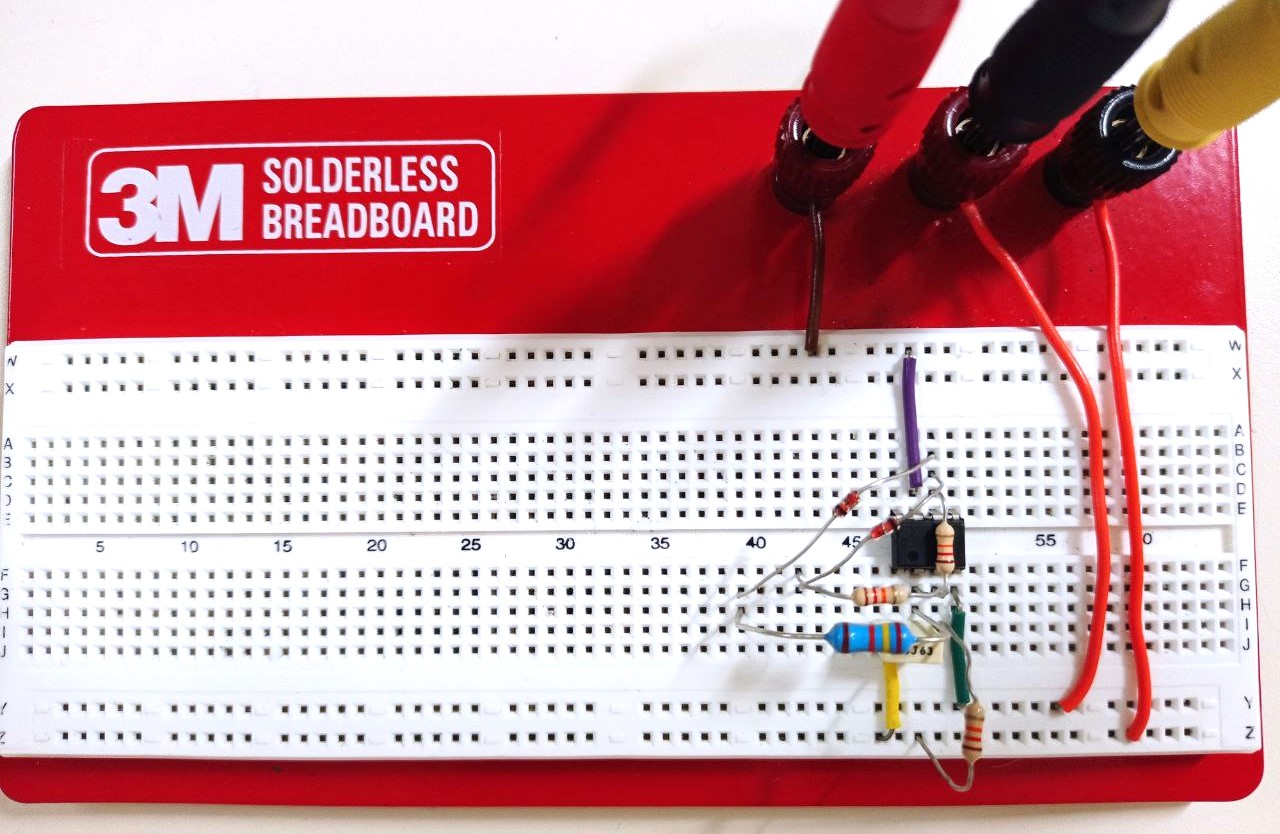
\includegraphics[height=6.2cm]{immagini/circuito4_1.jpg}
	\caption{Fotografia dell'oscillatore con duty cicle $\neq$ 50\% realizzato in laboratorio.}
	\label{figura:circuito4}
\end{figure}
%\begin{table}[h!]
%	\centering
%	\begin{tabular}{|c|c|c|}
	%		\cline{2-3} 
	%		\multicolumn{1}{c|}{} & \textbf{Valore nominale} & \textbf{Valore misurato}\\ 
	%		\hline
	%		$\mathbf{R_1}$ & \SI{18}{k\ohm} & \SI{17.977}{k\ohm} \\ 
	%		\hline
	%		$\mathbf{R_2}$ & \SI{33}{k\ohm} & \SI{37.630}{k\ohm} \\ 
	%		\hline
	%		$\mathbf{R_3}$ & \SI{56}{k\ohm} & \SI{54.742}{k\ohm} \\ 
	%		\hline
	%		$\mathbf{R_4}$ & $\displaystyle\mathrm{\SI{82}{k\ohm}+\SI{18}{k\ohm}=\SI{100}{k\ohm}}$ & $\displaystyle\mathrm{\SI{80.717}{k\ohm+}\SI{17.977}{k\ohm}=\SI{98.694}{k\ohm}}$ \\ 
	%		\hline
	%	\end{tabular}
%	\caption{Misure delle resistenze utilizzate nel raddrizzatore a semionda passivo.}
%	\label{table:misure1}
%\end{table}

%----------------------------------------------------------------------------------------

\end{document}
